%%%%%%%%%%%%%%%%%%%%%%%%%%%%%%%%%%%%%%%%%%%%%%%%%%%%%%%%%%%%
%%  This Beamer template was created by Cameron Bracken.
%%  Anyone can freely use or modify it for any purpose
%%  without attribution.
%%
%%  The current presentation created by Jeferson L. R. Souza (jefecomp) is based on the template created by Cameron Bracken. 
%%  
%%  Small modifications have been introduced and anyone is free to use such modified version.
%%
%% Last Modified: June 14, 2015.

\documentclass[xcolor=x11names,compress]{beamer}

%% General document %%%%%%%%%%%%%%%%%%%%%%%%%%%%%%%%%%%%%%%%%
\usepackage{graphicx}
\usepackage{tikz}
\usetikzlibrary{decorations.fractals}
%%%%%%%%%%%%%%%%%%%%%%%%%%%%%%%%%%%%%%%%%%%%%%%%%%%%%%

%Hyperref
\usepackage{hyperref}

%Multirow package
\usepackage{multirow} 

%Math packages
\usepackage{amsmath}
\usepackage{textcomp}



%% Beamer Layout %%%%%%%%%%%%%%%%%%%%%%%%%%%%%%%%%%
\useoutertheme[footline=authorinstitutetitle,subsection=false,shadow]{miniframes}
\useinnertheme{default}
\usefonttheme{professionalfonts}
\usepackage{palatino}

\setbeamerfont{title like}{shape=\scshape,series=\bfseries}
\setbeamerfont{frametitle}{shape=\scshape,series=\bfseries}

\setbeamercolor*{lower separation line head}{bg=Green3} 
\setbeamercolor*{upper separation line foot}{bg=Green3} 
\setbeamercolor*{normal text}{fg=black,bg=white} 
\setbeamercolor*{alerted text}{fg=black,bg=black!10} 
\setbeamercolor*{example text}{fg=black} 
\setbeamercolor*{structure}{fg=black}

 
\setbeamercolor*{palette tertiary}{fg=black,bg=black!3} 
\setbeamercolor*{palette quaternary}{fg=black,bg=black!10} 

%%%%%%%%%%%%%%%%%%%%%%%%%%%%%%%%%%%%%%%%%%%%%%%%%%

%%  user definitions and package declaration

\setbeamertemplate{blocks}[rounded] [shadow=true]

\setbeamertemplate{frametitle continuation}[from second][(Continuação)]


%%  declaring picture extensions and default path
\DeclareGraphicsExtensions{.png, .jpg, .pdf}
\graphicspath{{pictures/}}

%% Supporting source code lists
\usepackage{listings}
\lstset{breakatwhitespace,
language=Java,
columns=fullflexible,
keepspaces,
breaklines,
tabsize=3, 
showstringspaces=false,
extendedchars=true}

%Text position
\usepackage{textpos}
\setlength{\TPHorizModule}{128mm}
\setlength{\TPVertModule}{96mm}

\usepackage{array}


%Puting text and other float elements over pictures
\usepackage[percent]{overpic}


%% Hyperlinks over all the document
\usepackage{hyperref}

%% Controlling text alignment
\usepackage{ragged2e}

%% Framed text
\usepackage{framed}

%% Math packages
\usepackage{amsmath}

\begin{document}

\title[Introdução à Base de Dados \hskip27mm \insertframenumber / \inserttotalframenumber  \hskip33.2mm \inserttitlegraphic ]{Introdução à Base de Dados \\[4mm]
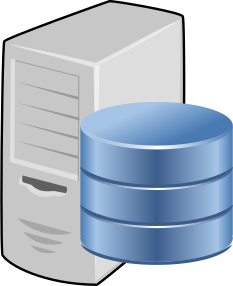
\includegraphics[keepaspectratio,width=.25\textwidth]{database-server}}
\author[@2018 Jeferson Souza, MSc (jefecomp) - All rights reserved.]{
	\textcolor{blue}{Prof. Jeferson Souza, MSc.} \\[1mm] 
	\textcolor{blue}{\textit{{\footnotesize (jefecomp) }}}\\[1.5mm]
	 \underline{{\footnotesize jefecomp.official@gmail.com}}
	 \vspace*{1mm}
}
\institute[]{\centering 
\includegraphics[keepaspectratio,width=.5\textwidth]{logo_udesc_joinville_horizontal_assinatura}
}

\date{}

\titlegraphic{
\includegraphics[keepaspectratio,width=.2\textwidth]{logo_udesc_joinville_horizontal_assinatura}}

%%%%%%%%%%%%%%%%%%%%%%%%%%%%%%%%%%%%%%%%%%%%%%%%%%%%%%
%%%%%%%%%%%%%%%%%%%%%%%%%%%%%%%%%%%%%%%%%%%%%%%%%%%%%%
\begin{frame}[plain,noframenumbering]
\titlepage
\end{frame}

%%%%%%%%%%%%%%%%%%%%%%%%%%%%%%%%%%%%%%%%%%%%%%%%%%%%%%
%%%%%%%%%%%%%%%%%%%%%%%%%%%%%%%%%%%%%%%%%%%%%%%%%%%%%%
\section{\scshape Definição}
\subsection{Base de dados}
\begin{frame}{Definição}

\only<1>{
\vspace*{-12mm}
}

O que é uma base de dados?

\only<1>{
\vspace*{10mm}
}

\begin{center}

\includegraphics[keepaspectratio,width=.2\textwidth]{database_symbol}
\end{center}

\only<2>{
\begin{itemize}

\item Uma base de dados pode ser definida como um conjunto de arquivos organizados de forma a armazenar dados relevantes para usuários/aplicações;

\item Novos dados podem ser inseridos na base de dados, assim como dados existentes podem ser atualizados, removidos, ou consultados.

\end{itemize}
}

\end{frame}

\begin{frame}{Definição}

Como esses dados podem ser manipulados?

\begin{center}
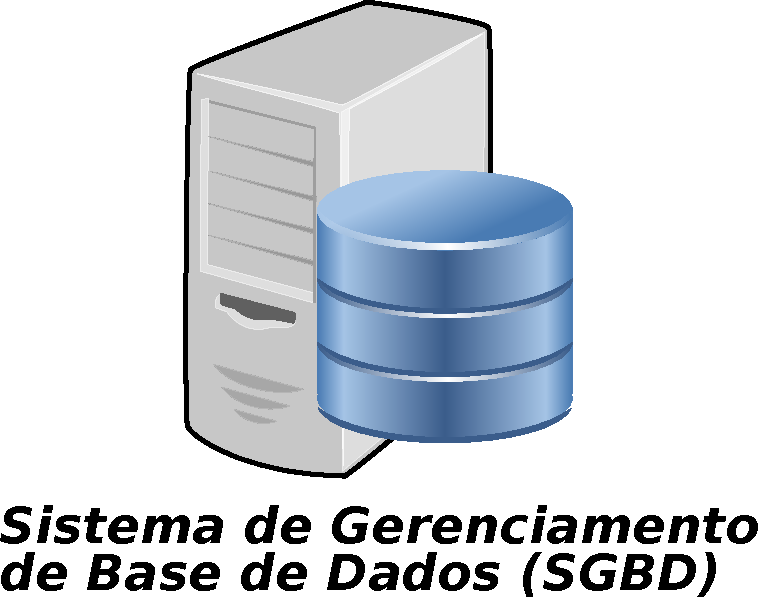
\includegraphics[keepaspectratio,width=.5\textwidth]{database-server-sgbd}
\end{center}

\centering Através de um Sistema de Gerenciamento de Base de Dados (SGBD).

\end{frame}


%%%%%%%%%%%%%%%%%%%%%%%%%%%%%%%%%%%%%%%%%%%%%%%%%%%%%%
%%%%%%%%%%%%%%%%%%%%%%%%%%%%%%%%%%%%%%%%%%%%%%%%%%%%%%
\section{\scshape História}
\subsection{História}

\begin{frame}{Um pouco de história ...}

\begin{itemize}
\itemsep 5mm
\item \underline{1950 e 1960}: Tempo das fitas magnéticas para armazenamento de dados. Operações de leitura e escrita das fitas eram realizadas sequencialmente;

\item \underline{1960 e 1970}: Introdução do uso de discos rígidos, melhorando consideravelmente a tarefa de acesso e processamento de dados. Dados podiam ser acessados diretamente. Nessa época foi publicado o artigo seminal que define o modelo relacional;

\end{itemize}

\end{frame}

\begin{frame}{Um pouco de história ...}

\begin{itemize}
\itemsep 5mm

\item \underline{1980}: Implementation do projeto R pela IBM, o qual criou um eficiente sistema de gerenciamento de base de dados relacional;

\item \underline{1990 (Início)}: Surge a linguagem de consulta estruturada SQL, do inglês Structured Query Language;

\end{itemize}

\end{frame}

\begin{frame}{Um pouco de história ...}

\begin{itemize}
\itemsep 5mm

\item \underline{1990}: Crescimento da World Wide Web, e como consequência crescimento na utlização de sistemas de gerenciamento de bases de dados;

\item \underline{2000}: Popularização no uso de bases de dados de código aberto (ex: PostgreSQL) e surgimento de novas tecnologias de bases de dados NoSQL. 

\end{itemize}

\end{frame}


%%%%%%%%%%%%%%%%%%%%%%%%%%%%%%%%%%%%%%%%%%%%%%%%%%%%%%
%%%%%%%%%%%%%%%%%%%%%%%%%%%%%%%%%%%%%%%%%%%%%%%%%%%%%%
\section{SGBD}
\subsection{SGBD}
\begin{frame}{Definição de SGBD}

\begin{center}
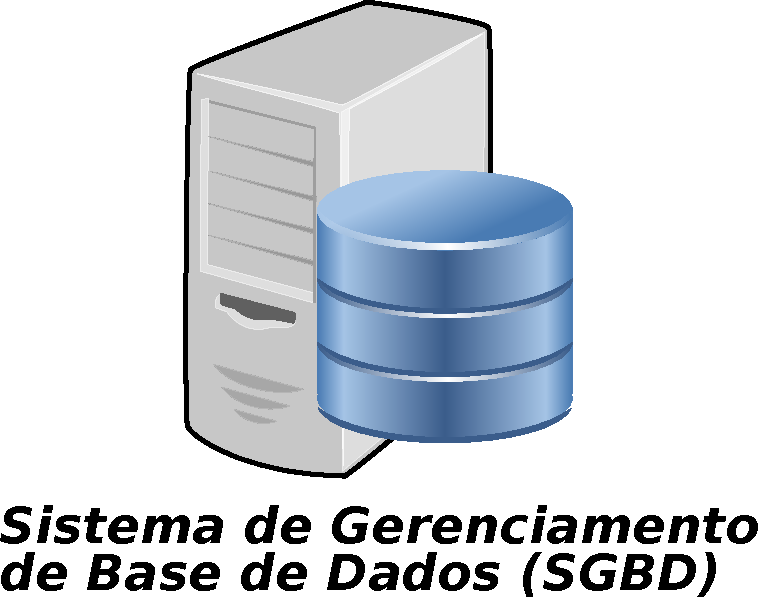
\includegraphics[keepaspectratio,width=.4\textwidth]{database-server-sgbd}
\end{center}

\begin{alertblock}{O que é um SGBD?}

Um SGBD é um conjunto de arquivos que armazenam dados interrelacionados, juntamente com um conjunto de programas que permitem manipular esses dados.

\end{alertblock}
\end{frame}

\begin{frame}{Onde estão os SGBDs?}

\only<1>{\vspace*{-15mm}}
\only<2>{\vspace*{-4.4mm}}

SGBDs são como os brasileiros: estão em todo o lado :-)!

\vspace*{3mm}

\begin{itemize}
\itemsep	5mm
\item Grandes corporações (ex: Google, Facebook, ...);

\item Diferentes segmentos: Indústria automotiva, indústria de entretenimento, bancos, entre outros.

\end{itemize}

\only<2-3>{
\begin{alertblock}{\centering Lembrem-se:}
\centering  Armazenamento de dados permite extração de informação. 
\end{alertblock}
}

\only<3>{
\begin{block}{}
\centering Informação é \underline{PODER}!!!
\end{block}
}
\end{frame}

\begin{frame}{Benefícios dos SGBDs}

\begin{itemize}

\item Reduzir redundância e inconsistência nos dados armazenados;

\item Melhoria no acesso aos dados - menos complicado e mais eficiente;

\item Interface única para acesso a diferentes tipos de dados;

\item Manutenção da intergridade dos dados;

\item Suporte ao acesso simultâneo dos dados;

\item Suporte a segurança dos dados.

\end{itemize}

\only<2>{
\begin{alertblock}{\centering O que eu ganho utilizando um SGBD?}
\centering Uma visão abstrata no acesso aos dados, sem a necessidade de saber os detalhes técnicos do armazenamento.
\end{alertblock}
}
\end{frame}

%%%%%%%%%%%%%%%%%%%%%%%%%%%%%%%%%%%%%%%%%%%%%%%%%%%%%%
%%%%%%%%%%%%%%%%%%%%%%%%%%%%%%%%%%%%%%%%%%%%%%%%%%%%%%
\section[Abstração]{Níveis de Abstração}
\subsection{Abstração}
\begin{frame}{Níveis de Abstração}
 
 \label{lb:abstraction_levels}

\begin{center}

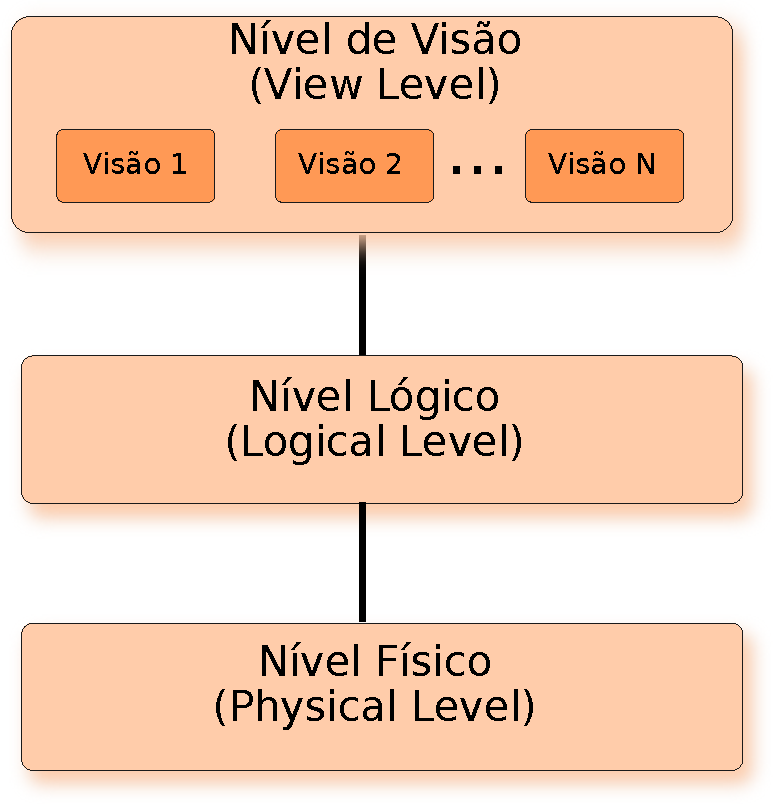
\includegraphics[keepaspectratio,width=.5\textwidth]{sgbd_abstraction_levels}

\end{center}

\vspace*{-2mm}
\centering {\tiny *Baseada na figura 1.1 do livro ``Database Systems"~\cite{SilberchatzEtAl2011}}.

\end{frame}

\begin{frame}{Nível Físico (Physical Level)}

\begin{center}

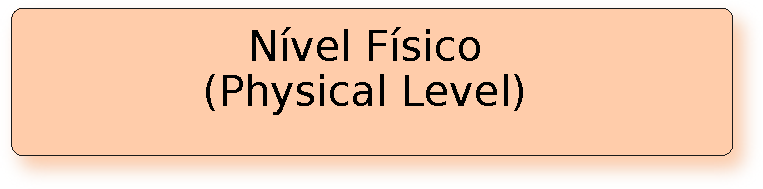
\includegraphics[keepaspectratio,width=.5\textwidth]{sgbd_physical_level}

\end{center}
 
\begin{block}{}
Detalhes de armazenamento dos dados são especificados no nível físico. O nível físico define as estruturas de dados necessárias para armazenamento, e organização dos dados no dispositivo de armazenamento (ex: disco rígido);
\end{block}

\end{frame}

\begin{frame}{Nível Lógico (Logical Level)}

\begin{center}

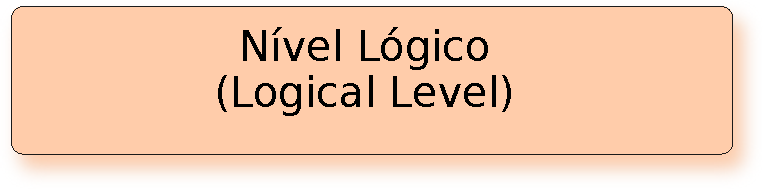
\includegraphics[keepaspectratio,width=.5\textwidth]{sgbd_logical_level}

\end{center}
 
\begin{block}{}
Primeiro nível de abstração dos dados armazenados no nível físico. No nível lógico são especificados os relacionamentos e restrições na definição dos dados. Nesse nível é definido o que realmente será armazenado.
\end{block}

\end{frame}

\begin{frame}{Nível de Visão (View Level)}

\begin{center}

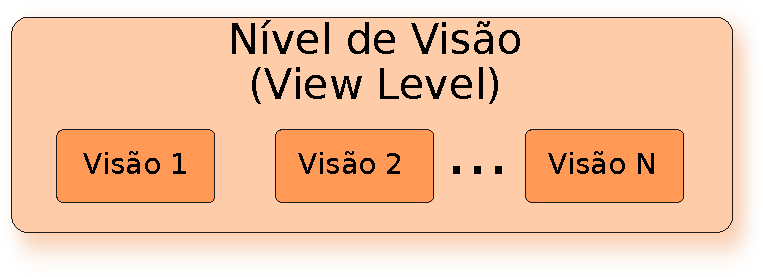
\includegraphics[keepaspectratio,width=.5\textwidth]{sgbd_view_level}

\end{center}
 
\begin{block}{}
Define diferentes visões da mesma base de dados. Além disso pode especificar restrições de acesso, ou seja, um determinado usuário pode ter permissão de acesso somente a uma pequena parte da base de dados.
\end{block}

\end{frame}


%%%%%%%%%%%%%%%%%%%%%%%%%%%%%%%%%%%%%%%%%%%%%%%%%%%%%%
%%%%%%%%%%%%%%%%%%%%%%%%%%%%%%%%%%%%%%%%%%%%%%%%%%%%%%
\section[Modelos]{Modelos de Dados}
\subsection{Modelo de Dados}
\begin{frame}{O que é um Modelo de Dados?}

\only<1>{
Um modelo de dados é uma forma de descrever dados ou informação nos trẽs níveis de abstração: físico, lógico, e visão.
}

\only<2>{

Possui 3 principais características:

\begin{itemize}
\itemsep 5mm 
\item Estrutura dos dados;

\item Operações sobre os dados;

\item Restrições sobre os dados.

\end{itemize}
}
\end{frame}

\begin{frame}{Modelos de dados}

\begin{itemize}
\itemsep 5mm

\item Relacional;

\item Entidade Relacionamento (E-R);

\item Baseado em objetos;

\item Objeto-Relacional;

\item Semi-estruturado.

\end{itemize}


Existem diferentes modelos de dados na literatura. Vamos nos concentrar (por agora) no \underline{modelo de dados Relacional}.

\end{frame}


%%%%%%%%%%%%%%%%%%%%%%%%%%%%%%%%%%%%%%%%%%%%%%%%%%%%%%
%%%%%%%%%%%%%%%%%%%%%%%%%%%%%%%%%%%%%%%%%%%%%%%%%%%%%%
\section{Modelo Relacional}
\subsection{Modelo Relacional}
\begin{frame}{O que é o modelo de dados relacional?}

\begin{itemize}
\itemsep 5mm
\item Consiste em uma forma estruturada de representar dados, e as relações entre esses dados;

\item Dados são representados em tabelas, e uma tabela define um domínio específico desses dados;

\item As colunas das tabelas representam as suas características (e tipos de dados).


\end{itemize}

\end{frame}

\begin{frame}{Tabelas}

\begin{center}
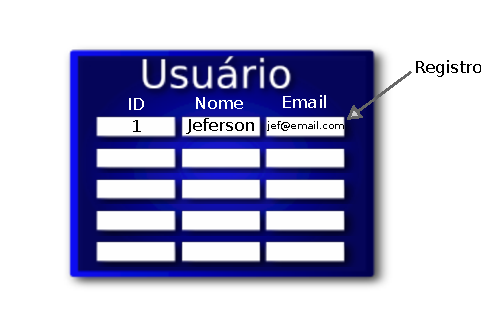
\includegraphics[keepaspectratio,width=.6\textwidth]{db_tables}
\end{center}

\begin{block}{}
Um registro é uma linha em uma tabela que possui valores atribuídos a cada uma das colunas especificadas. Esses valores podem ser nulos (ausência de valor).
\end{block}

\end{frame}

\begin{frame}{Identificando registros unicamente}

Por que é importante identificar registros em uma tabela de forma única?

\begin{itemize}
\itemsep 5mm

\item Evitar inserção de dados repetidos (diminuir redundância);

\item Permitir o estabelecimento de relações com outras tabelas;

\item Permitir uma consulta mais eficiente dos dados.

\end{itemize}

\begin{block}{}
\centering A identificação única de um registro em uma tabela é denominada \underline{chave primária}.
\end{block}

\end{frame}

\begin{frame}{Chave primária (primary key)}

\only<1>{
\begin{itemize}
\itemsep 5mm

\item Identifica únicamente um registro em uma tabela;

\item Pode ser composta por uma ou mais colunas de uma tabela. Ex: id, \{nome, telefone\};

\item Uma boa chave primária praticamente não se altera com o passar do tempo. Exemplo: identificadores sequenciais gerados automaticamente.

\end{itemize}
}

\only<2>{

Exemplo:

\begin{center}
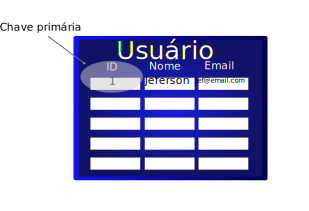
\includegraphics[keepaspectratio,width=0.7\textwidth]{primary_key}
\end{center}
}
\end{frame}

\begin{frame}{Candidatos à chave}

\only<1>{
\vspace*{-15mm}
O que são candidatos à chave (candidate keys)?

\vspace*{15mm}

\begin{block}{}
Candidatos a chave são colunas (ou combinação de colunas) de uma tabela que podem (além da chave primária) identificar unicamente um registro da tabela. Ex: CPF, email, \{nome, telefone\}.
\end{block}
}

\only<2>{
Exemplo:

\begin{center}
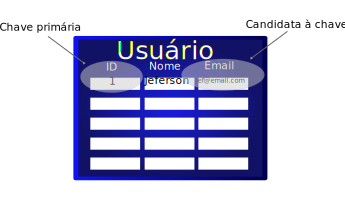
\includegraphics[keepaspectratio,width=.7\textwidth]{candidate_key}
\end{center}
}

\only<3>{
\vspace*{-15mm}
Por que é importante identificar colunas candidatas à chave?

\vspace*{15mm}
\begin{block}{}
Colunas candidatas à chave são ótimos elementos para gerar indices (tópico abordado mais a frente no curso).
\end{block}

}
\end{frame}

\begin{frame}{Chave estrangeira (foreign key)}

\only<1>{
\begin{itemize}
\itemsep 5mm

\item Referencia a chave primária de outra tabela;

\item Usar chaves estrangeiras é a forma de estabelecer relações entre tabelas no modelo relacional.

\end{itemize}
}

\only<2>{
Exemplo:

\begin{center}
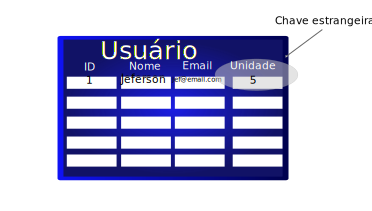
\includegraphics[keepaspectratio,width=.8\textwidth]{foreign_key}
\end{center}
}


\end{frame}

\begin{frame}{Relacionamento Um para Um (One to One)}

\begin{center}
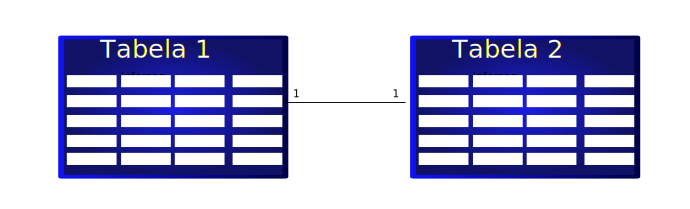
\includegraphics[keepaspectratio,width=\textwidth]{relation_one_to_one}
\end{center}

\begin{block}{}
\centering A chave estrangeira é definida do lado da relação que fizer mais sentido para consulta dos dados.
\end{block}

\end{frame}

\begin{frame}{Relacionamento Um para Muitos (One to Many)}

\begin{center}
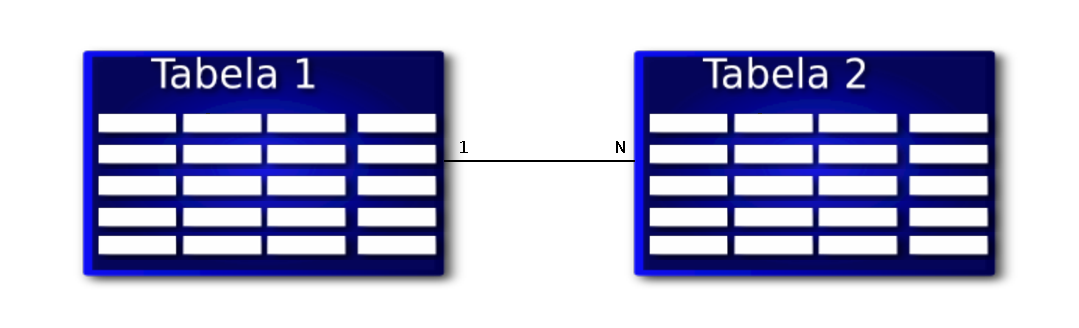
\includegraphics[keepaspectratio,width=\textwidth]{relation_one_to_many}
\end{center}

\begin{block}{}
\centering A chave estrangeira é definida do lado N da relação.
\end{block}

\end{frame}

\begin{frame}{Relacionamento Muitos para Muitos (Many to Many)}

\begin{center}
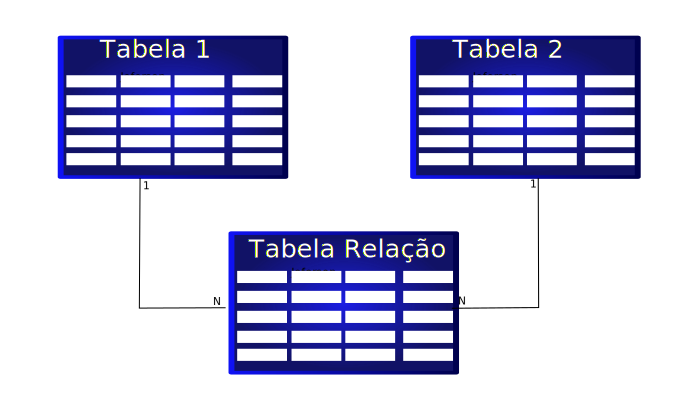
\includegraphics[keepaspectratio,width=.6\textwidth]{relation_many_to_many}
\end{center}

\begin{block}{}

\centering A chave estrangeira de ambas as tabelas é defina na tabela de relação. Asumindo que PK1 é a chave primária da tabela 1, e PK2 a chave primária da tabela 2, podemos definir a chave primária da tabela de relação como sendo:

 \centering \{ PK1, PK2 \}
\end{block}

\end{frame}

\begin{frame}[allowframebreaks]{Schema de base de dados}

\begin{itemize}
\itemsep 5mm

\item Define todos os elementos presentes em uma base de dados (Estutura);

\item Especificado com auxílio da linguagem de definição de dados, do inglês Data Definition Language (DDL) (sublinguagem do SQL);

\item Depois de completamente definido, mudanças em um dado schema praticamente não ocorrem.

\item Três tipos de schema: Físico, Lógico, e Visão. Seguem a mesma organização dos níveis de abstração apresentados a partir do slide~\ref{lb:abstraction_levels}.  

\end{itemize}

\begin{alertblock}{\centering \underline{Instância de um schema}}
\centering Uma instância de um schema  representa toda a coleção de dados desse schema em um dado instante de tempo.
\end{alertblock}

\end{frame}

\begin{frame}{Exemplo de schema de base de dados}

\begin{center}
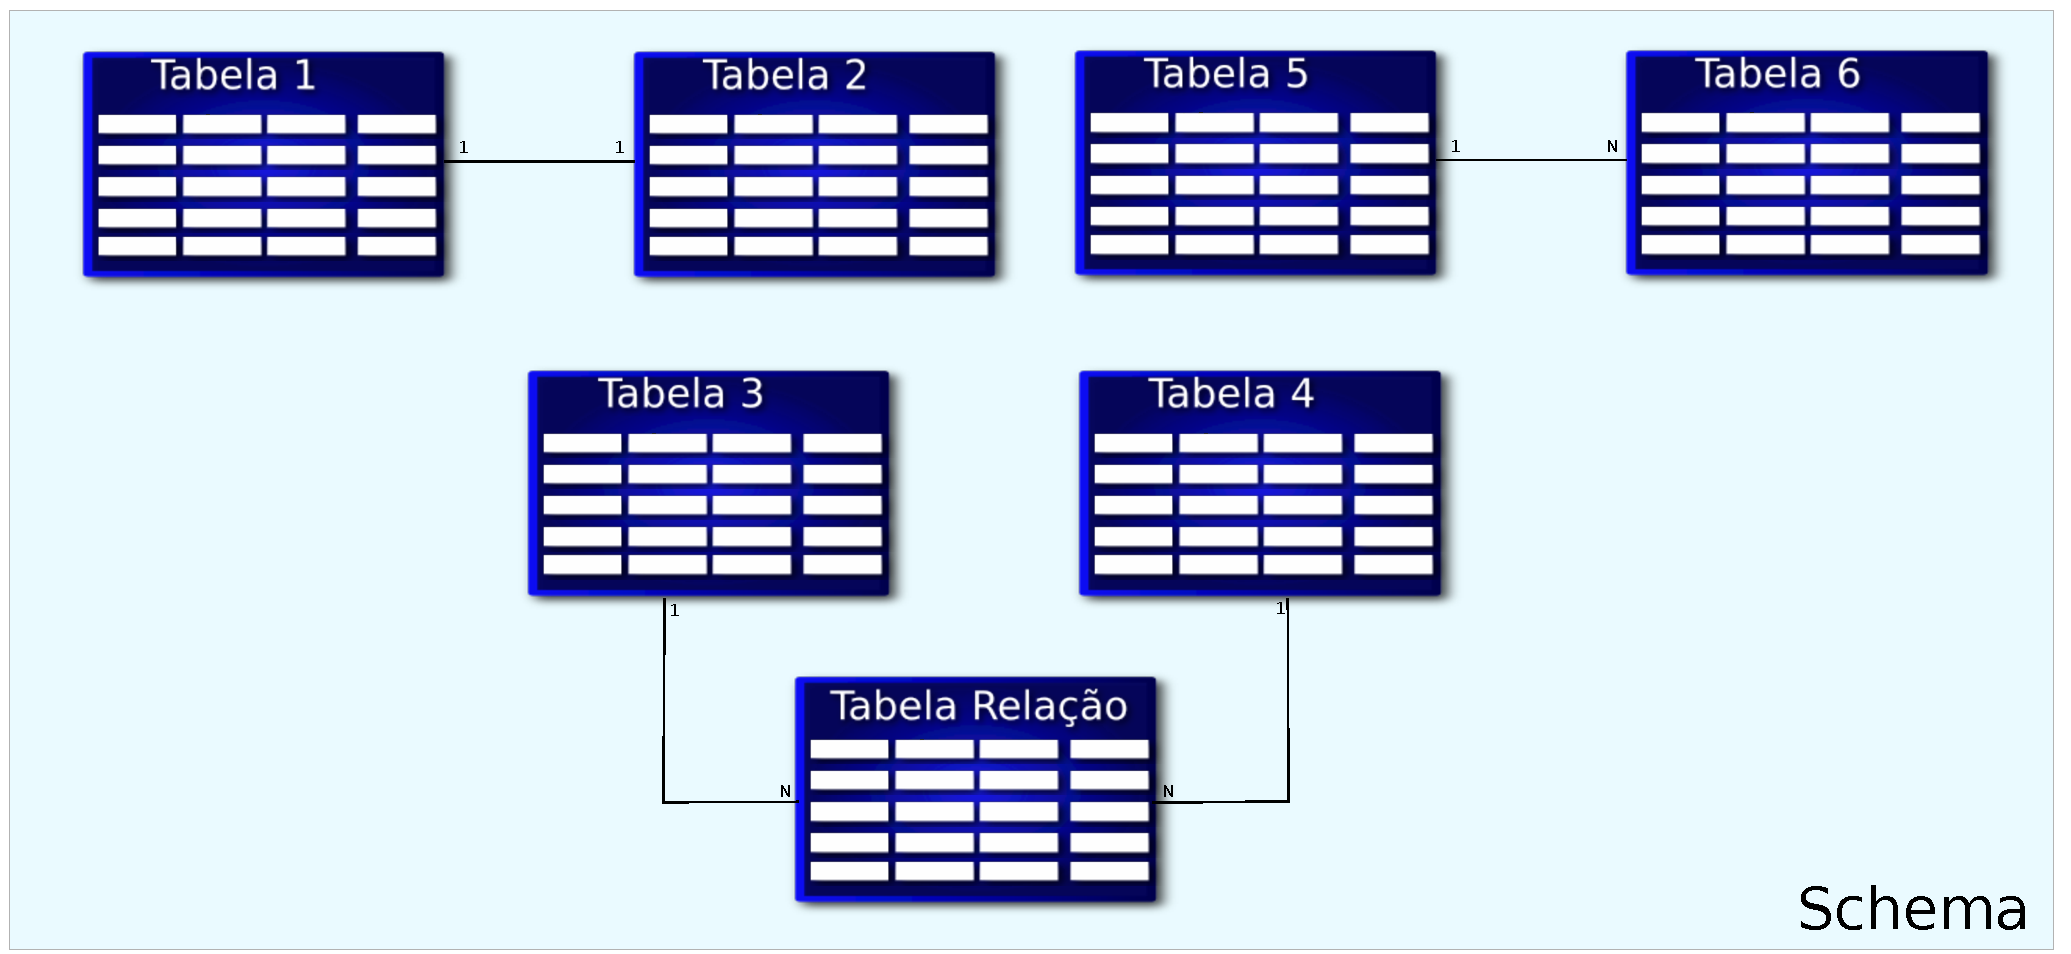
\includegraphics[keepaspectratio,width=\textwidth]{schema}
\end{center}

\end{frame}

\begin{frame}[allowframebreaks]{Exercício de Fixação}

Descreva o esquema de uma base de dados para um sistema bancário. Por agora vamos modelar somente as seguintes entidades: Cliente, Endereço, Conta, Operação, e Movimentos. Diferentemente da aula anterior, onde desenhamos graficamente as tabelas e suas relações, utilize o diagrama de Entidade Relacionamento (E-R) para modelar o esquema proposto. Além disso, identifique claramente na sua modelagem os seguintes aspectos:

\begin{itemize}
\itemsep 5mm

\item Chave primária de cada entidade;

\item Chave estrangeira das relações estabelecidas;

\item Atributos candidatos à chave em cada uma das entidades.

\end{itemize}

Depois de realizada a modelagem, responda (Sim ou Não) a seguinte pergunta: \\[5mm]

A estratégia utilizada para converter o diagrama E-R para tabelas no banco de dados foi representar cada entidade como uma uma tabela?

\end{frame}

%%%%%%%%%%%%%%%%%%%%%%%%%%%%%%%%%%%%%%%%%%%%%%%%%%%%%%
%%%%%%%%%%%%%%%%%%%%%%%%%%%%%%%%%%%%%%%%%%%%%%%%%%%%%%
\section[Projeto BD]{Projeto de Banco de Dados}
\subsection{Projeto Banco de Dados}
\begin{frame}{Fases de Projeto}

\begin{itemize}

\item Levantamento inicial de requisitos;

\item Desenho conceitual;

\item Especificação dos requisitos funcionais;

\item Desenho lógico;

\item Desenho físico.

\end{itemize}

\end{frame}

\begin{frame}{Fase de levantamento inicial de requisitos}

\begin{itemize}
\itemsep 5mm

\item Iteração com especialistas no domínio dos dados que o projeto da base de dados está inserido;

\item Iteração com usuários da base de dados;

\item Identificação e levantamento de requisitos proveniente da iteração com ambos especialistas e usuários;

\item Produção da \underline{especificação dos requisitos de usuário};

\item Remoção de redundâncias existentes nos requitos especificados.

\end{itemize}

\end{frame}

\begin{frame}{Fase de desenho conceitual}

\begin{itemize}
\itemsep 5mm

\item Criação do \underline{schema conceitual} da base de dados, o qual especifica a estrutura dos dados e suas relações;

\item Validação do schema conceitual criado para confirmar que todos os requisitos levantados estão presentes no modelo conceitual, e não tem conflitos;

\item Remoção de eventuais redundâncias de dados presentes no schema conceitual criado.

\end{itemize}

\end{frame}

\begin{frame}{Fase de Especificação de Requisitos Funcionais}

\begin{itemize}
\itemsep 5mm

\item Descrição das \underline{operações e transações} que poderão ser executadas sobre os dados;

\item Operações podem incluir inserção, atualização, remoção e busca de dados;

\item Verificação do schema conceitual visando atestar que, o mesmo, encontra-se em conformidade com os requisitos funcionais descritos.

\end{itemize}

\end{frame}

\begin{frame}{Fase de Desenho Lógico}

\begin{itemize}
\itemsep 5mm

\item Nesta fase, acontece o mapeamento do modelo conceitual mais abstrato (alto-nível) para um modelo concreto de dados;

\item O resultado é a implementação do schema conceitual na base de dados.

\end{itemize}

\end{frame}

\begin{frame}{Fase de Desenho Físico}

\begin{itemize}
\itemsep 5mm

\item Descrição de estruturas de dados (à nível físico) que permitam o armazenamento e acesso eficiente da implementação do schema conceitual realizada no nível lógico.

\end{itemize}

\begin{alertblock}{\centering Observação}
Normalmente não é necessário especificar estruturas de dados para auxiliar no armazenamento do schema conceitual implementado ao nível lógico. Porém, em alguns casos, pode ser necessário adicionar novas estruturas de dados no nível físico para permitir tanto o armazenamento, quanto o acesso eficiente dos dados no nível físico. 
\end{alertblock}

\end{frame}

%%%%%%%%%%%%%%%%%%%%%%%%%%%%%%%%%%%%%%%%%%%%%%%%%%%%%%
%%%%%%%%%%%%%%%%%%%%%%%%%%%%%%%%%%%%%%%%%%%%%%%%%%%%%%
\section{Arquitetura}
\subsection{Arquitetura}

\begin{frame}{Tipos de arquitetura de banco de dados}

\vspace*{-6mm}
\begin{center}
\begin{columns}[T]
\begin{column}{.5\textwidth}
\centering 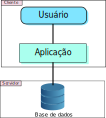
\includegraphics[keepaspectratio,width=.6\textwidth]{two_tier_db_architecture}

\centering Arquitetura de duas camadas

\end{column}

\begin{column}{.5\textwidth}

\centering 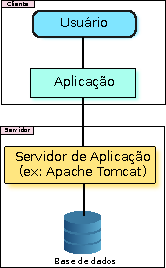
\includegraphics[keepaspectratio,width=.6\textwidth]{three_tier_db_architecture}

\centering Arquitetura de três camadas
\end{column}

\end{columns}
\end{center}

\centering {\tiny *Baseada na figura 1.6 do livro ``Database Systems"~\cite{SilberchatzEtAl2011}}.
\end{frame}

%%%%%%%%%%%%%%%%%%%%%%%%%%%%%%%%%%%%%%%%%%%%%%%%%%%%%%
%%%%%%%%%%%%%%%%%%%%%%%%%%%%%%%%%%%%%%%%%%%%%%%%%%%%%%
\section{}

\begin{frame}[plain,allowframebreaks,noframenumbering]{Bibliografia}

\begin{thebibliography}{Garcia-MolinaEtAl, 2008}

\bibitem[Garcia-MolinaEtAl, 2008]{Garcia-MolinaEtAl2008}

Garcia-Molina, H. and Ullman, J. D. and Widom, J.

\newblock{{\em ``Database Systems: The Complete Book}. 2nd edition. Prentice Hall, 2008.}

\bibitem[SilberchatzEtAl, 2011]{SilberchatzEtAl2011}

Silberschatz, A. and Korth, H.F. and Sudarshan, S.

\newblock	{{\em ``Database Systems"}. 6th edition. McGrawHill, 2011.}

\end{thebibliography}


\end{frame}
\begin{frame}[plain,noframenumbering]

\begin{center}

\includegraphics[keepaspectratio, width=.8\textwidth]{happycat-end}
\end{center}
\end{frame}


\end{document}